\documentclass[a4paper,12pt]{article}
\usepackage[T2A]{fontenc}
\usepackage[utf8]{inputenc}
\usepackage[english, russian]{babel}
\usepackage{minted}
\usepackage{verbatim}
\usepackage{graphicx}
\usepackage{caption}
\usepackage{subcaption}
\usepackage[left=2.5cm,right=2.5cm,top=2cm,bottom=2cm]{geometry}

\newenvironment{longlisting}{\captionsetup{type=listing}}{}

\newenvironment{pseudolisting}
 {\begin{minipage}{\linewidth}\vspace*{\topsep}}
 {\vspace*{\topsep}\end{minipage}}

\begin{document}

\begin{titlepage}
  \begin{center}
    \large
     
    \textbf{Федеральное государственное автономное образовательное учреждение высшего образования}
    \vspace{0.5cm}
 
    НАЦИОНАЛЬНЫЙ ИССЛЕДОВАТЕЛЬСКИЙ УНИВЕРСИТЕТ \\ "ВЫСШАЯ ШКОЛА ЭКОНОМИКИ"
    \vspace{0.5cm}
     
    Московский институт электроники и математики имени А. Н. Тихонова 
     
    Программа "Прикладная математика"
    \vfill
     
     
    Нигматуллин Роман Максимович
    \vfill
 
    \textsc{Лаборатная работа №7}\\[5mm]
     
    {\LARGE Решение ОДУ\\[2mm]
    }
  \bigskip
     
    3 курс, группа БПМ203
\end{center}
\vfill
 

 
\hfill\begin{flushright}
  \textbf{Преподаватель:}\\
  Брандышев Петр Евгеньевич
\end{flushright}%
\vfill
 
\begin{center}
  Москва, 2021 г.
\end{center}
\end{titlepage}


\tableofcontents

\section{Общие функции для ЛР на Python}
\begin{longlisting}
\inputminted{python}{src/ode.py}
\end{longlisting}

\section{Решение ОДУ и оценка погрешности методом Рунге (7.1.16)}
\subsection{Формулировка задачи}
Найти приближенное решение задачи Коши для ОДУ 1 порядка. Оценить погрешность решения.
\begin{enumerate}
	\item Задать исходные данные: функцию $f$ правой части, начальное значение $y_0$.
	\item Найти приближенное решение задачи Коши с шагом $h=0.1$ по явному методу Эйлера.
	\item Написать программу для поиска приближенного решения с шагом $h=0.1$ по методу Рунге-Кутты 4 порядка точности.
	\item Найти решение аналитически.
	\item Построить таблицы значений приближенных и точного решений, построить графики.
	\item Оценить погрешность двумя способами: по формуле $\varepsilon = max|y(t_i) - y_i|$ и по правилу Рунге (по правилу двойного пересчета).
	\item Выяснить, при каком $h^*$ решение по методу Эйлера имеет такую же погрешность, как решение при помощи метода Рунге-Кутты с шагом $h=0.1$.
\end{enumerate}

\subsection{Вариант}
$$ f(t, y) = - \frac{y}{t} + 3t $$

$$ t_0 = 1; \space T = 2; \space y_0 = 1 $$

\subsection{Аналитическое решение}
Дано ОДУ:
$$ \frac{dy}{dt} = - \frac{y}{t} + 3t $$
Сначала решим уравнение:
$$ \frac{dy}{dt} + \frac{y}{t} = 0 $$ 
Разделим переменные и получим общее решение:
$$ \frac{t}{dt} = - \frac{y}{dy} $$ 

$$ y(t) = \frac{C}{t} $$ 
Полное решение:
$$ \frac{C'}{t} + (-\frac{C}{t^2}) + \frac{C}{t^2} = 3t $$

$$ C' = 3t^2 $$

$$ C = t^3 + C_2 $$

$$ y = t^2 + t^{-1} $$

$$ y(1) = 1 $$

$$ y = t^2 $$

\subsection{Код на Python}

\begin{longlisting}
\inputminted{python}{src/eyler_vs_rk.py}
\end{longlisting}

\subsection{Вывод программы}
За приемлемое число итераций и время работы достигнуть того же уровня точности, как в методе Рунге-Кутты, не получилось.
Максимально достигнутая точность представлена в выводе ниже:
\begin{longlisting}
\inputminted{python}{output/eyler_vs_rk.txt}
\end{longlisting}

\subsection{Графики результирующих решений}
\begin{figure}[H]
	\centering
	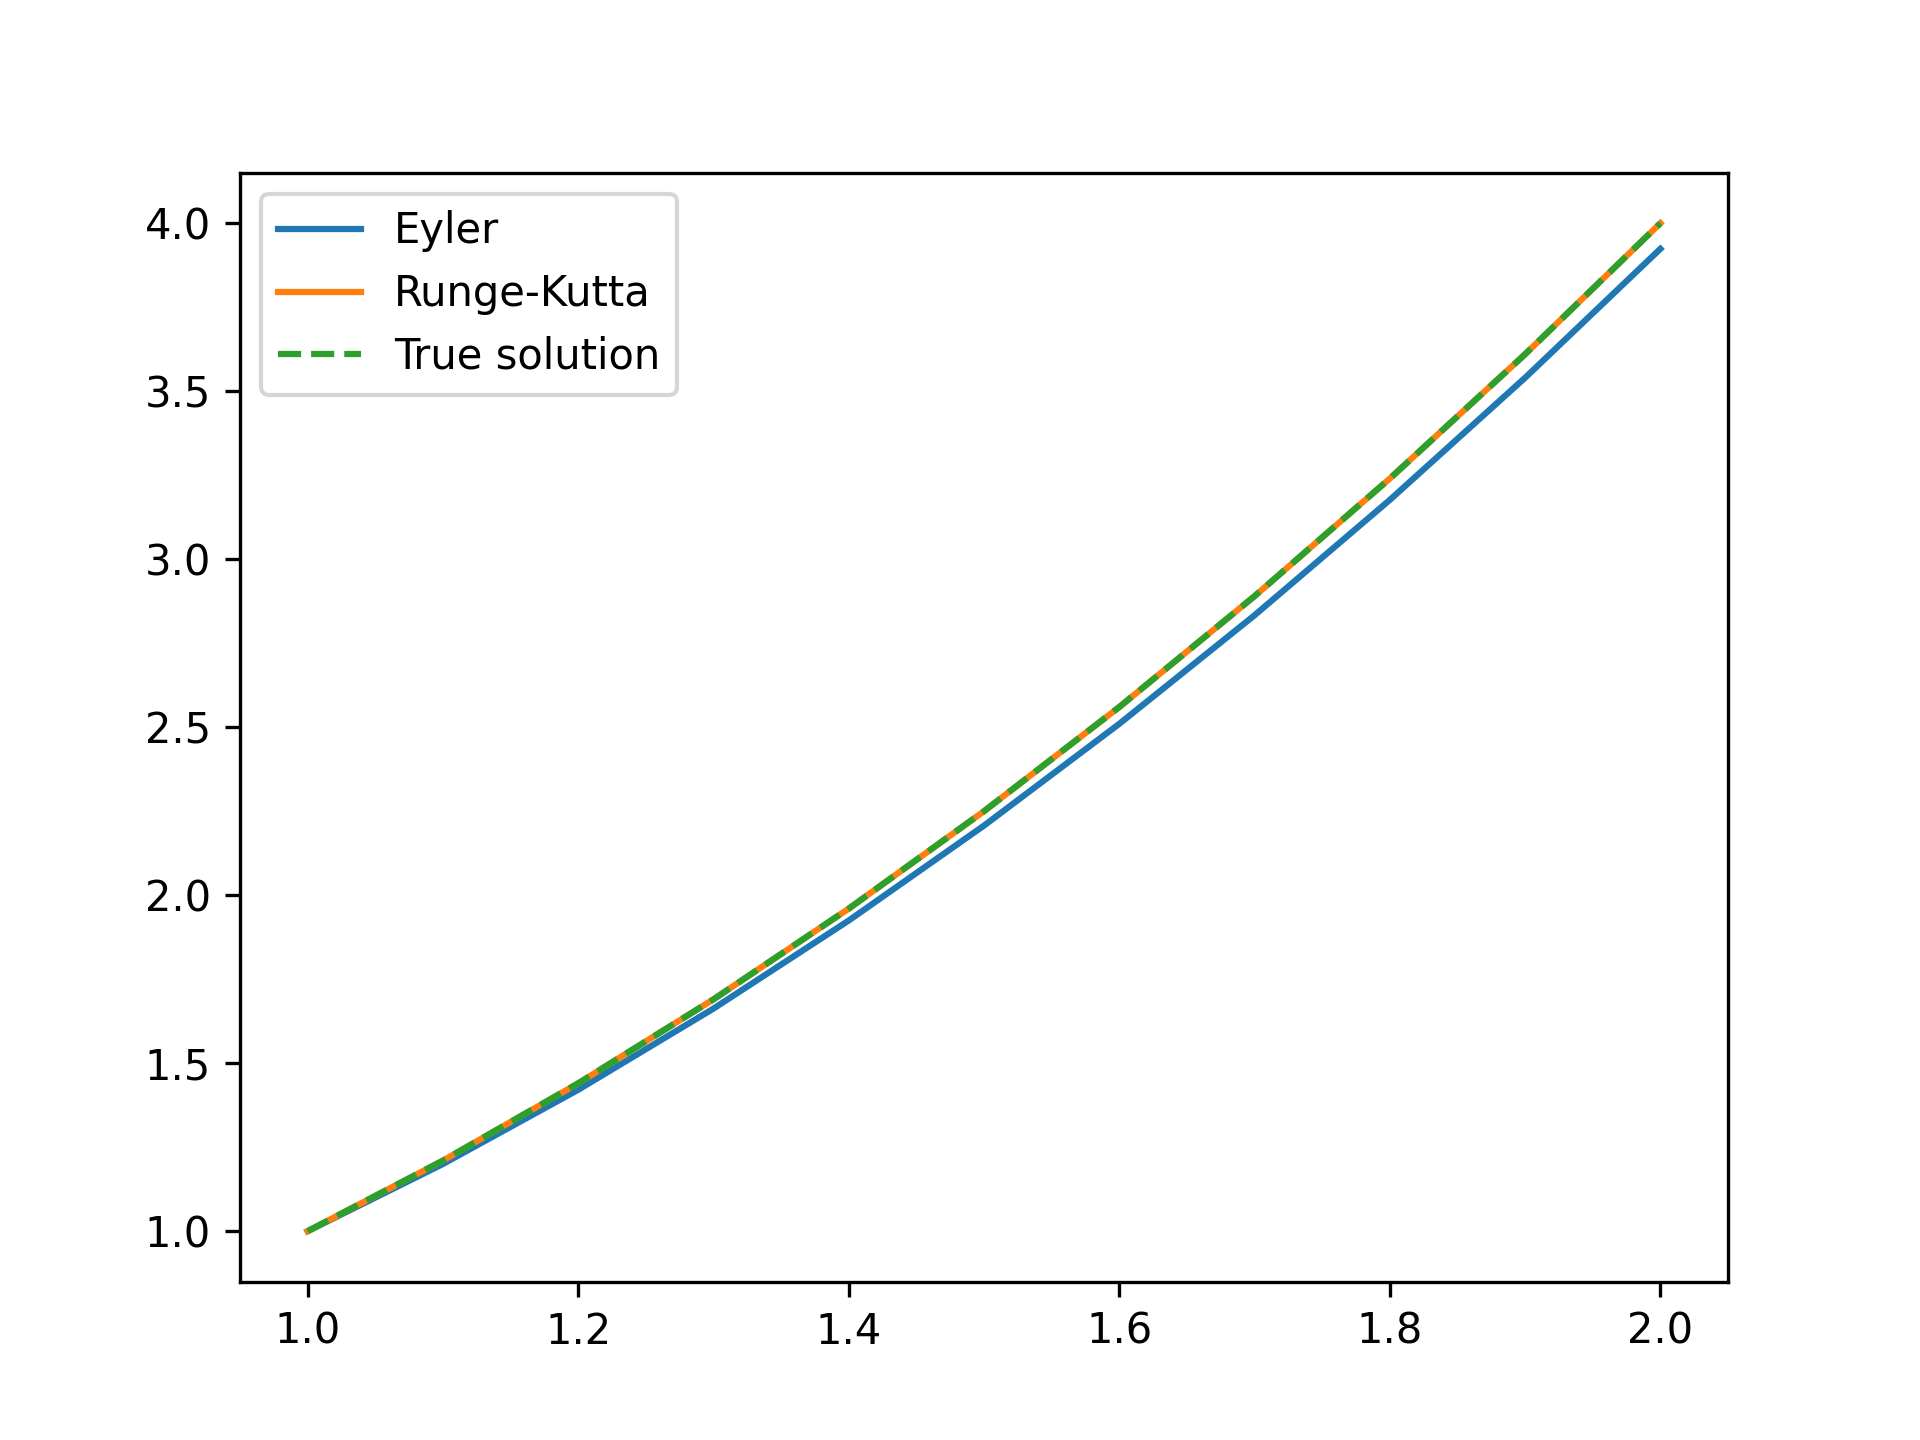
\includegraphics[width=\linewidth]{plots/eyler_vs_rk.png}
	\caption{Графики решений уравнения}
	\label{fig:eyler_rk}
\end{figure}

\section{Уточненное решение ОДУ по методу Рунге (7.3.6)}
\subsection{Формулировка задачи}
Решить приближенно задачу Коши для ОДУ 1 порядка, используя метод Рунге-Кутты 4 порядка и метод в варианте с использованием шагов $h, \frac{h}{2}$. Оценить погрешность по правилу Рунге, вычислить уточненное решение. Построить графики приближенных решений и графики уточненных решений.

\subsection{Вариант}
Метод - Экстраполяционный метод Адамса 3 порядка.
$$ f(t, y) = -ty + (t-1) e^t y^2 $$

$$ t_0 = 0; \space T = 1; \space y_0 = 1 $$

\subsection{Код на Python}

\begin{longlisting}
	\inputminted{python}{src/adams_vs_rk.py}
\end{longlisting}

\subsection{Графики результирующих решений}
\begin{figure}[H]
	\centering
	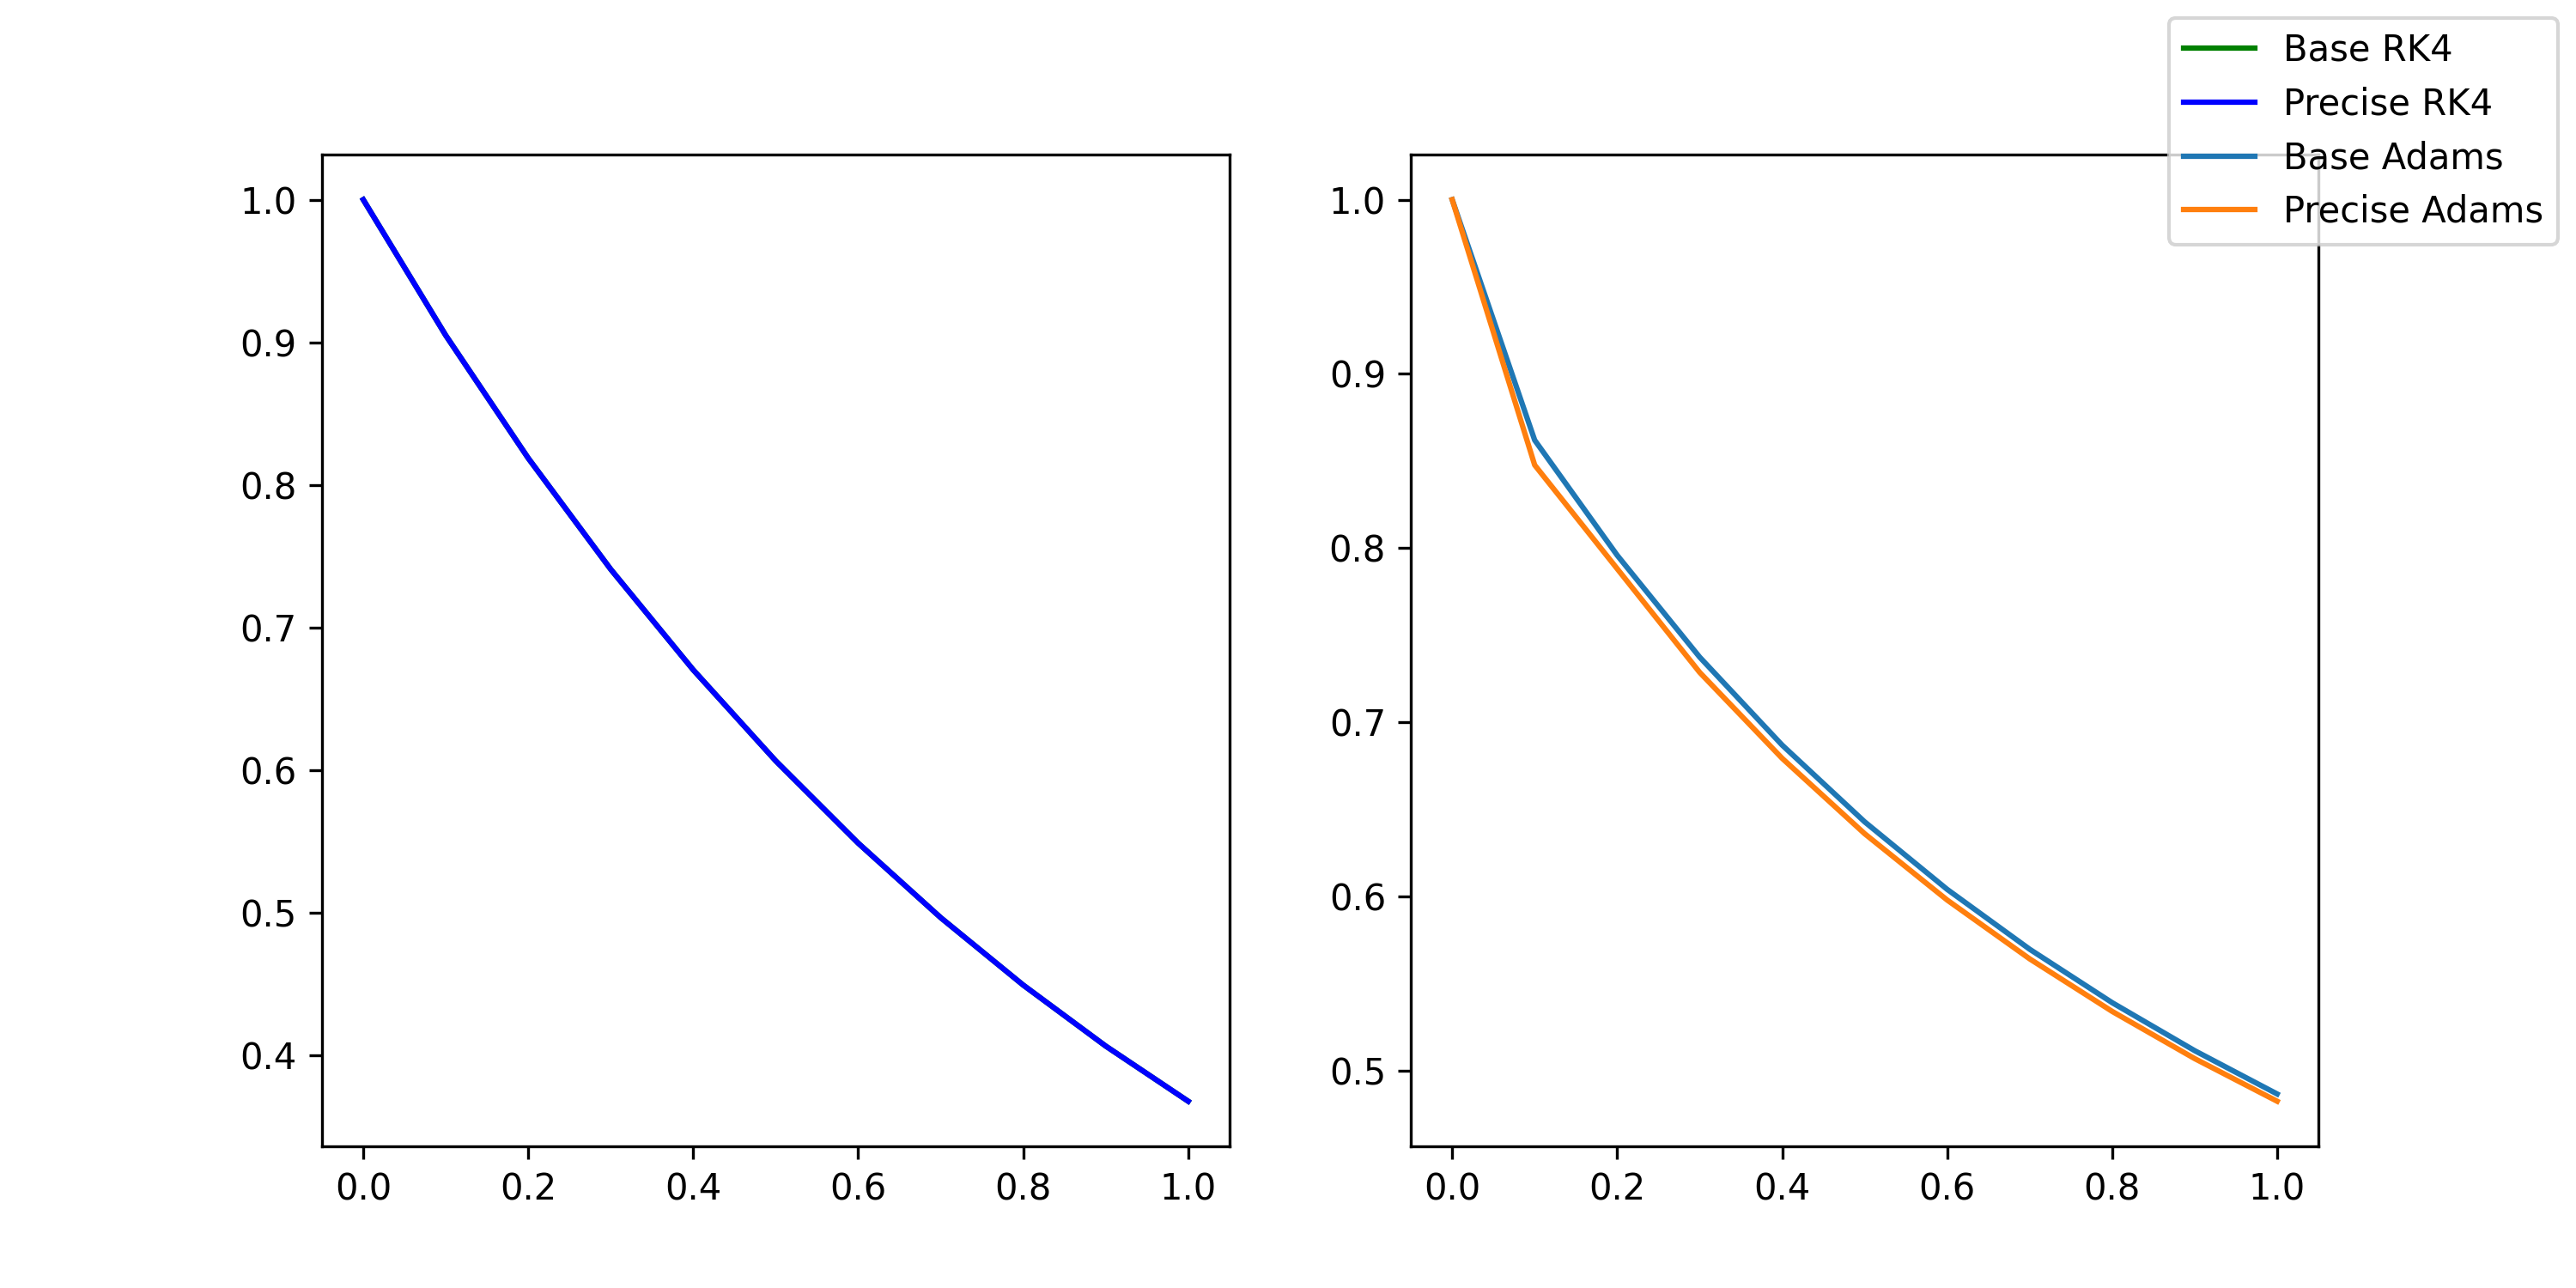
\includegraphics[width=\linewidth]{plots/adams_vs_rk.png}
	\caption{Графики решений уравнения}
	\label{fig:adams_rk}
\end{figure}

\section{Уточненное решение ОДУ по методу Рунге (7.3.6)}

\subsection{Формулировка задачи}
Решить приближенно задачу Коши для ОДУ 1 порядка с помощью метода в индивидуальном варианте с точностью $\varepsilon = 10^{-4}$, использовать алгоритм автоматического выбора шага.
В результате работы должен создаваться файл с вектором значений приближенного решения, а также значения шага $h$, при котором достигается точность. Программа по запросу должна выдавать таблицу значений или график найденного решения.

\subsection{Вариант}
Метод - Модифицированный метод Эйлера 2 порядка.

$$ f(t, y) = -\frac{1}{3}y \sqrt{t} + \frac{2}{3}y^2 sin{t} $$
 
$$ t_0 = 2; \space T = 10; \space y_0 = 2.2 $$

\subsection{Код на Python}

\begin{longlisting}
	\inputminted{python}{src/adaptive_step.py}
\end{longlisting}

\subsection{Вывод программы}

\begin{longlisting}
	\inputminted{python}{output/adaptive_step.txt}
\end{longlisting}


\subsection{Графики результирующих решений}

\begin{figure}[H]
	\centering
	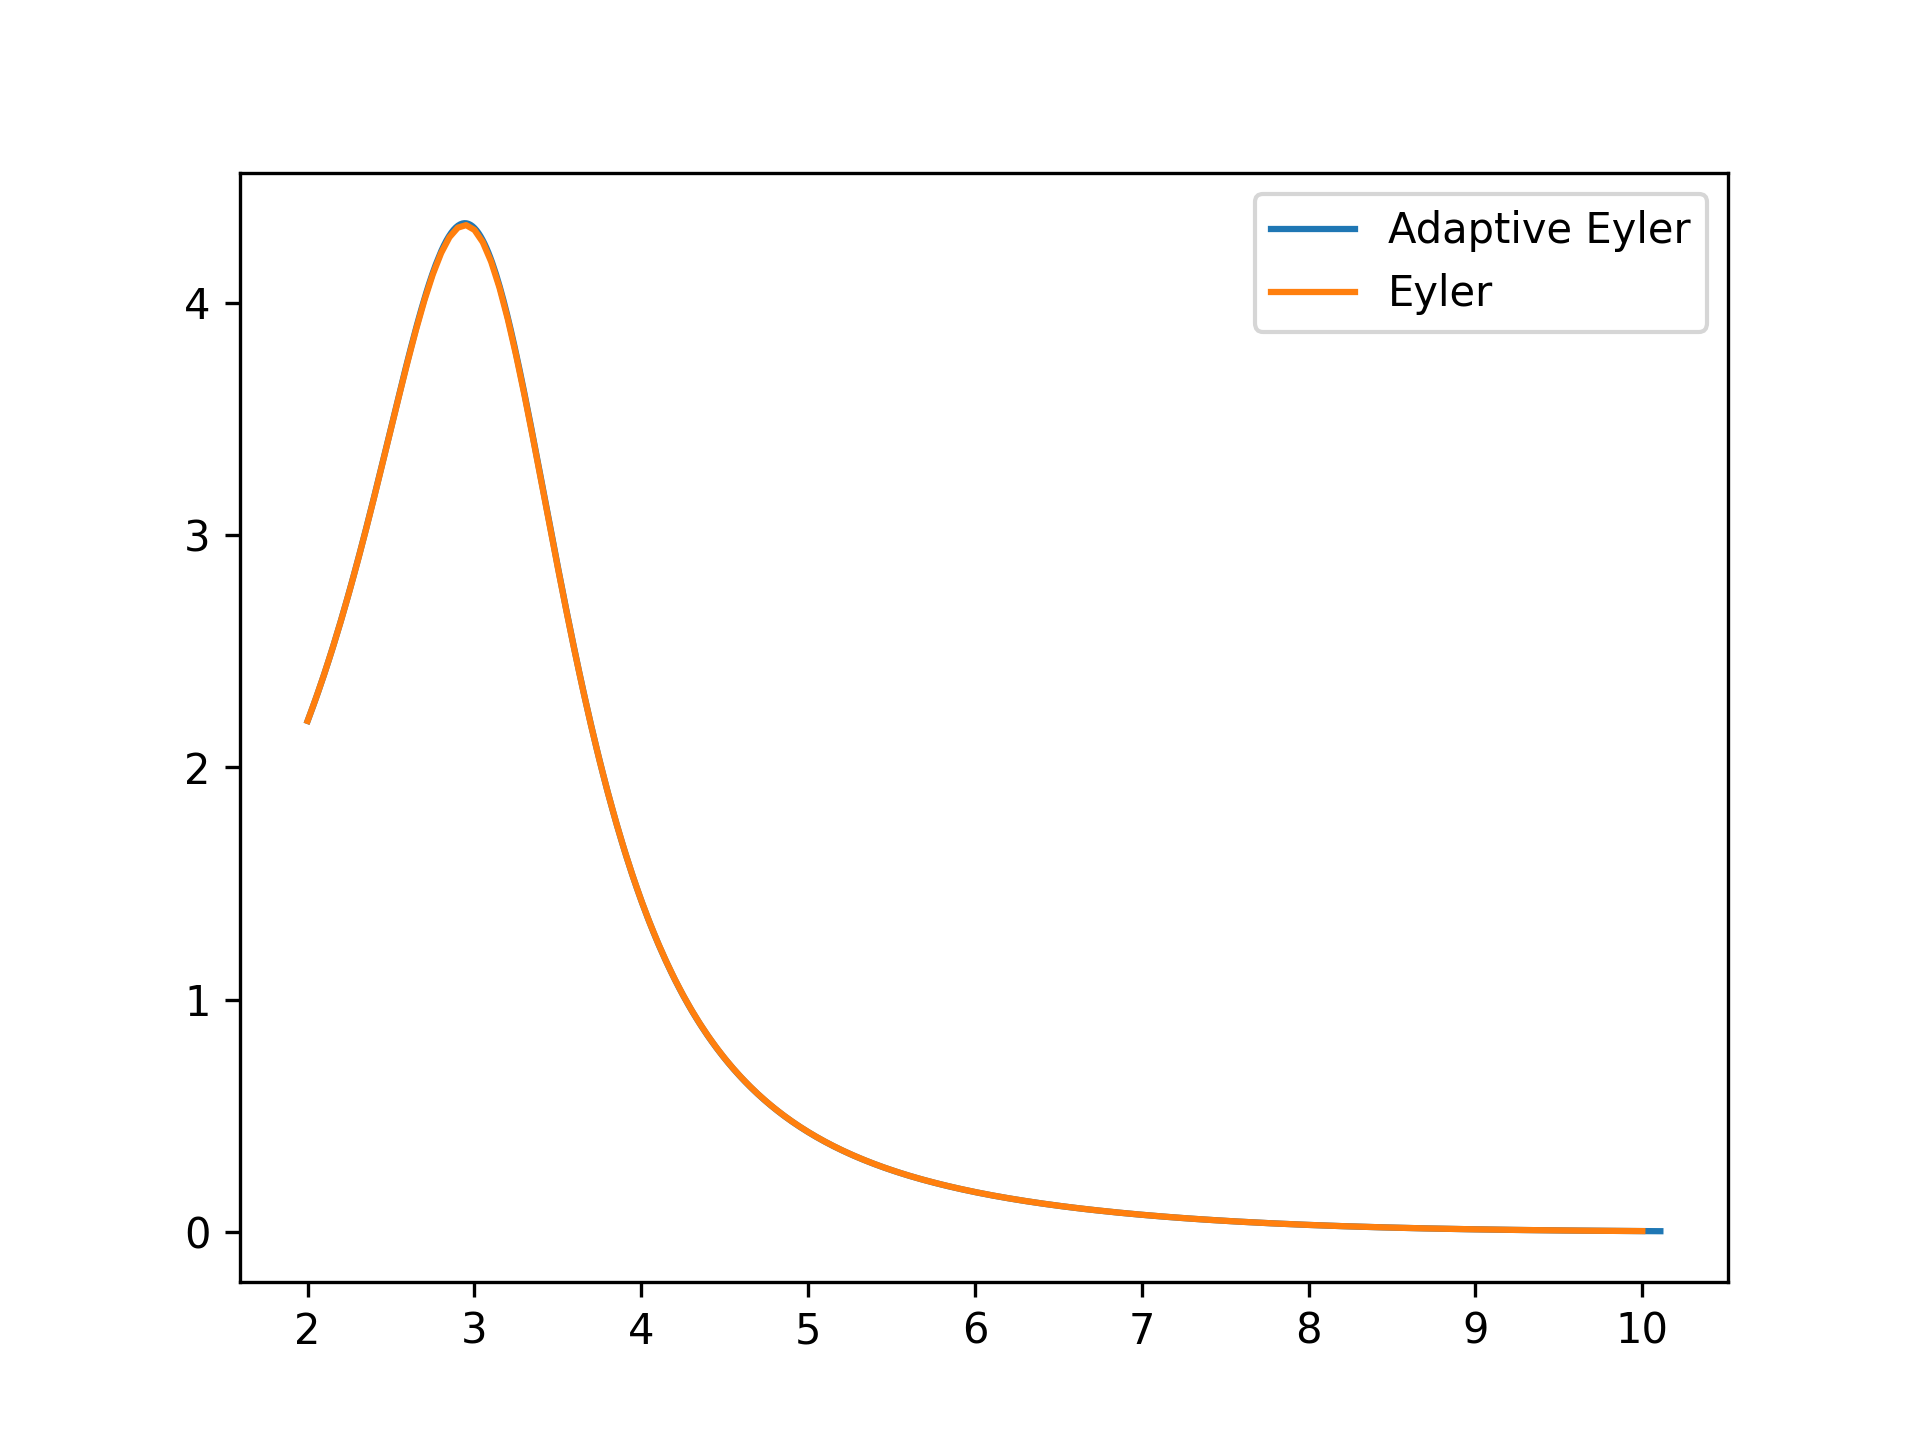
\includegraphics[width=\linewidth]{plots/adaptive_step.png}
	\caption{Графики решений уравнения}
	\label{fig:adams_rk}
\end{figure}



\end{document}